\documentclass{beamer}
\title{Mnesia ACL schema migration}
\author{Ilya Averyanov}
\institute{EMQX}
\date{2021}
\usetheme{emqx}
\usepackage{listings}
\usepackage{color}
\usepackage{graphicx}
\usepackage{xcolor}
\usepackage{hyperref}
\definecolor{href}{rgb}{0,0,0.9375}
\hypersetup{
    pdfborderstyle={/S/U/W 1}, % underline links instead of boxes
    colorlinks=true,
    urlcolor=href
}
\lstset{frame=tb,
  aboveskip=3mm,
  belowskip=3mm,
  showstringspaces=false,
  columns=flexible,
  basicstyle={\small\ttfamily},
  numbers=none,
  numberstyle=\tiny\color{gray},
  keywordstyle=\color{blue},
  commentstyle=\color{dkgreen},
  stringstyle=\color{mauve},
  breaklines=true,
  breakatwhitespace=false,
  tabsize=2
}


\begin{document}

\frame{\titlepage}

\begin{frame}
    \frametitle{Initial problem}
    \framesubtitle{100\% High CPU on v4.3.6 vs v4.2.6}

    \begin{itemize}
        \item \href{https://github.com/emqx/emqx/issues/5506}{https://github.com/emqx/emqx/issues/5506}
        \item User has ~5000 clients
        \item Clients connect and subscribe simultaneously
        \item Small CPU usge peak on 4.2
        \item Long lasting 100\% CPU flatline on 4.3
    \end{itemize}
\end{frame}

\begin{frame}
    \frametitle{Initial problem}
    \framesubtitle{v4.3.6, reproduced by the user}

    \begin{center}
        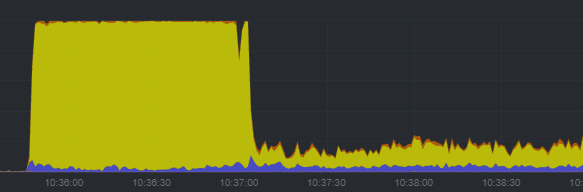
\includegraphics[width=10cm, keepaspectratio]{images/initial-4.3.png}
    \end{center}
\end{frame}

\begin{frame}
    \frametitle{Initial problem}
    \framesubtitle{v4.2.6 comparison}

    \begin{center}
        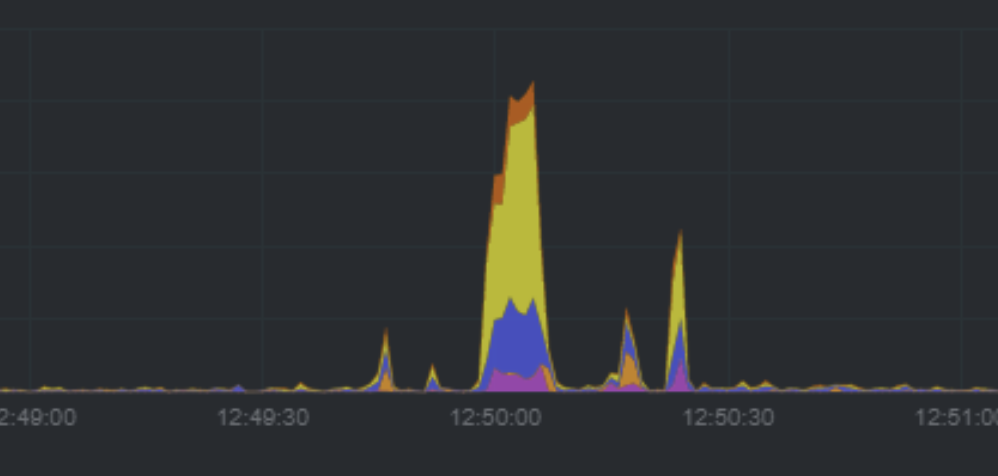
\includegraphics[width=10cm, keepaspectratio]{images/initial-4.2.png}
    \end{center}
\end{frame}

\begin{frame}
    \frametitle{Steps to reproduce}

    \begin{itemize}
        \item Write a convenience script to create MQTT users and their ACLs
        \item Create ~5000 MQTT users with ACLs
        \item Run \lstinline{emqtt-bench} with \lstinline{-c 5000 -i 0}
    \end{itemize}
\end{frame}

\begin{frame}
    \frametitle{Steps to reproduce}

    \begin{center}
        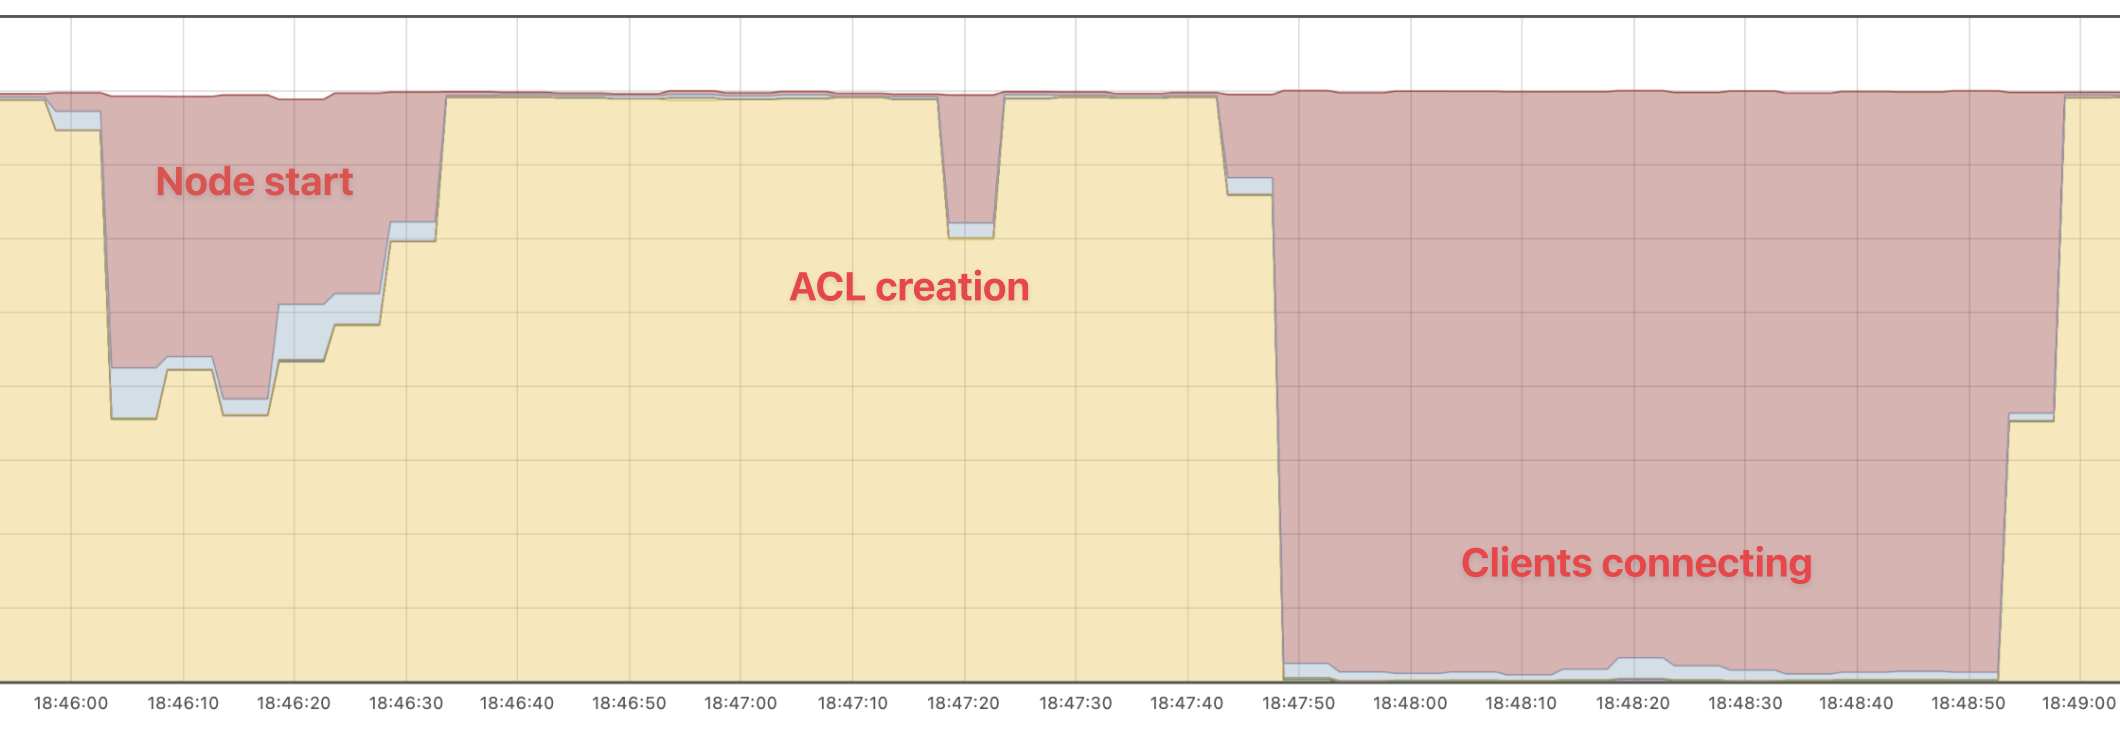
\includegraphics[width=10cm, keepaspectratio]{images/reproduce.png}
    \end{center}
\end{frame}

\begin{frame}
    \frametitle{So what's the problem?}

    \begin{center}
        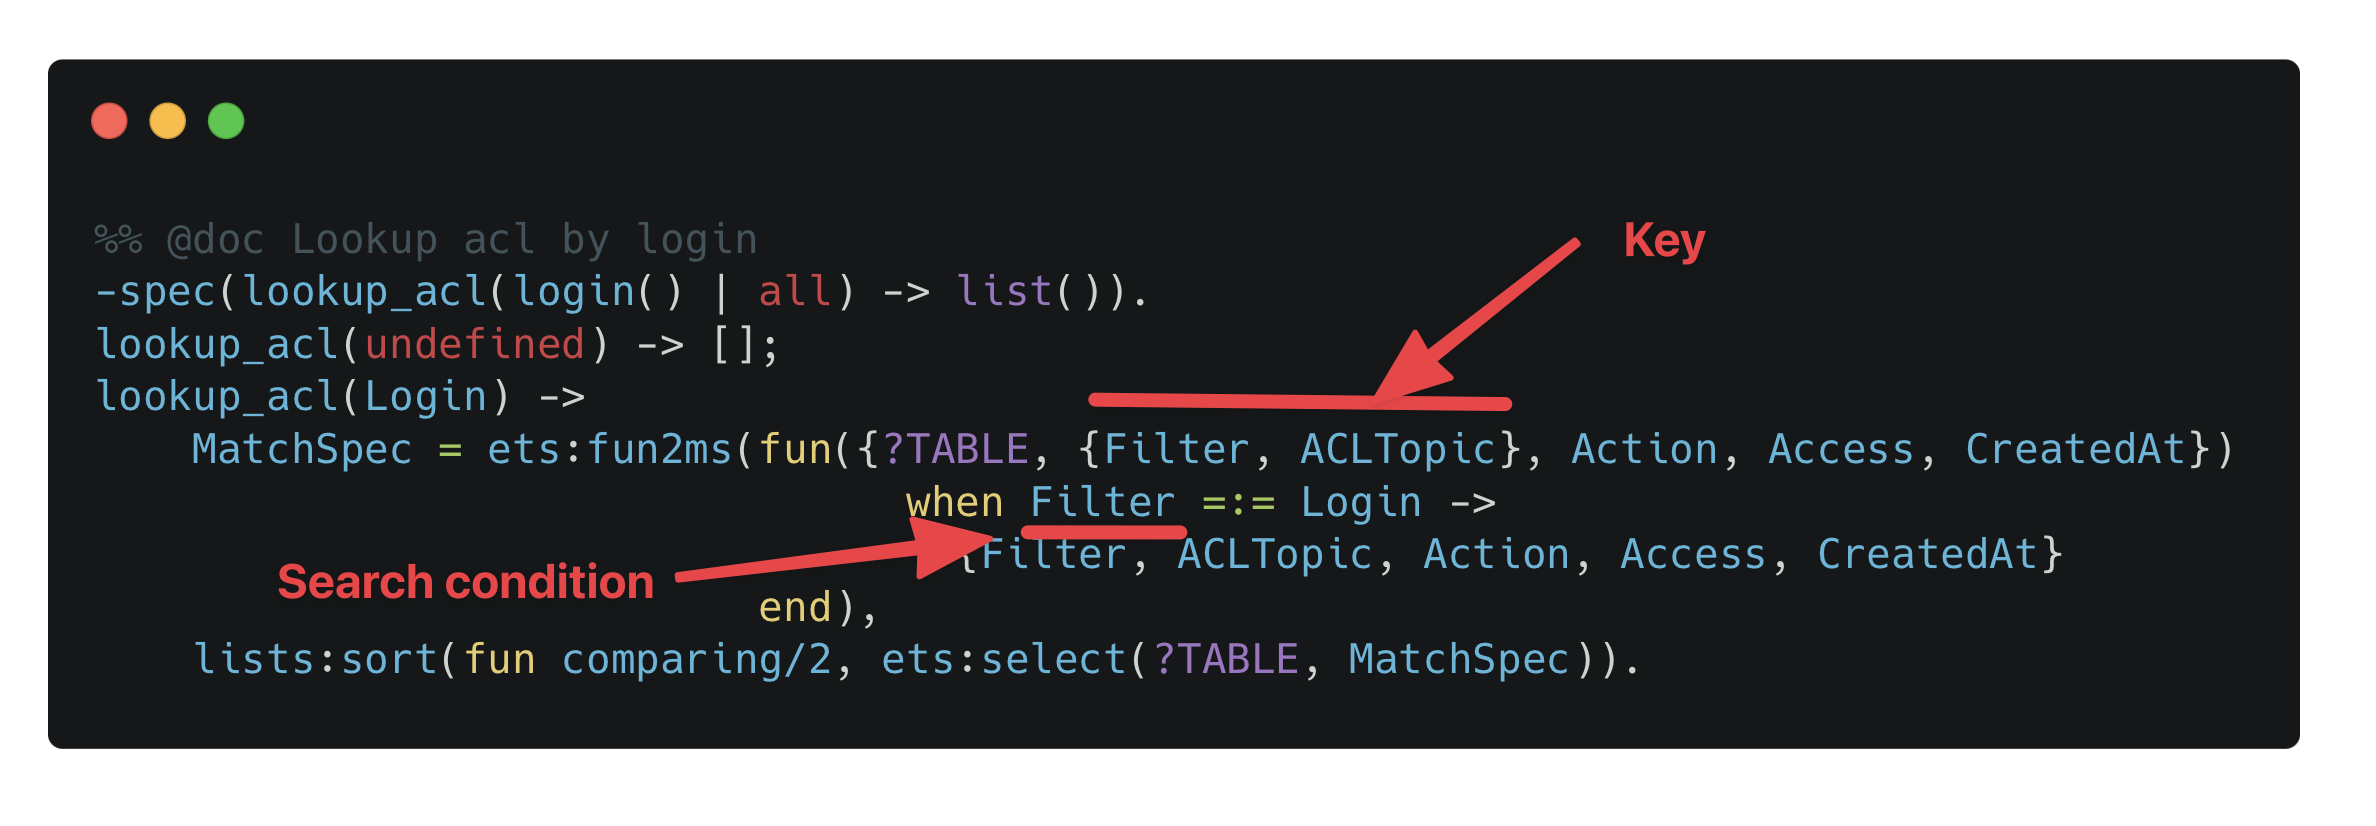
\includegraphics[width=10cm, keepaspectratio]{images/old-lookup-code.png}
    \end{center}
\end{frame}

\begin{frame}
    \frametitle{So what's the problem?}

    \begin{itemize}
        \item We have \textbf{bag} table with \lstinline{\{UserId, Topic\}} key
        \item We search by \lstinline{UserId}, i.e. part of the key
        \item So full \lstinline{ets} scan is done every time
    \end{itemize}
\end{frame}

\begin{frame}
    \frametitle{So what's the problem?}

    \begin{center}
        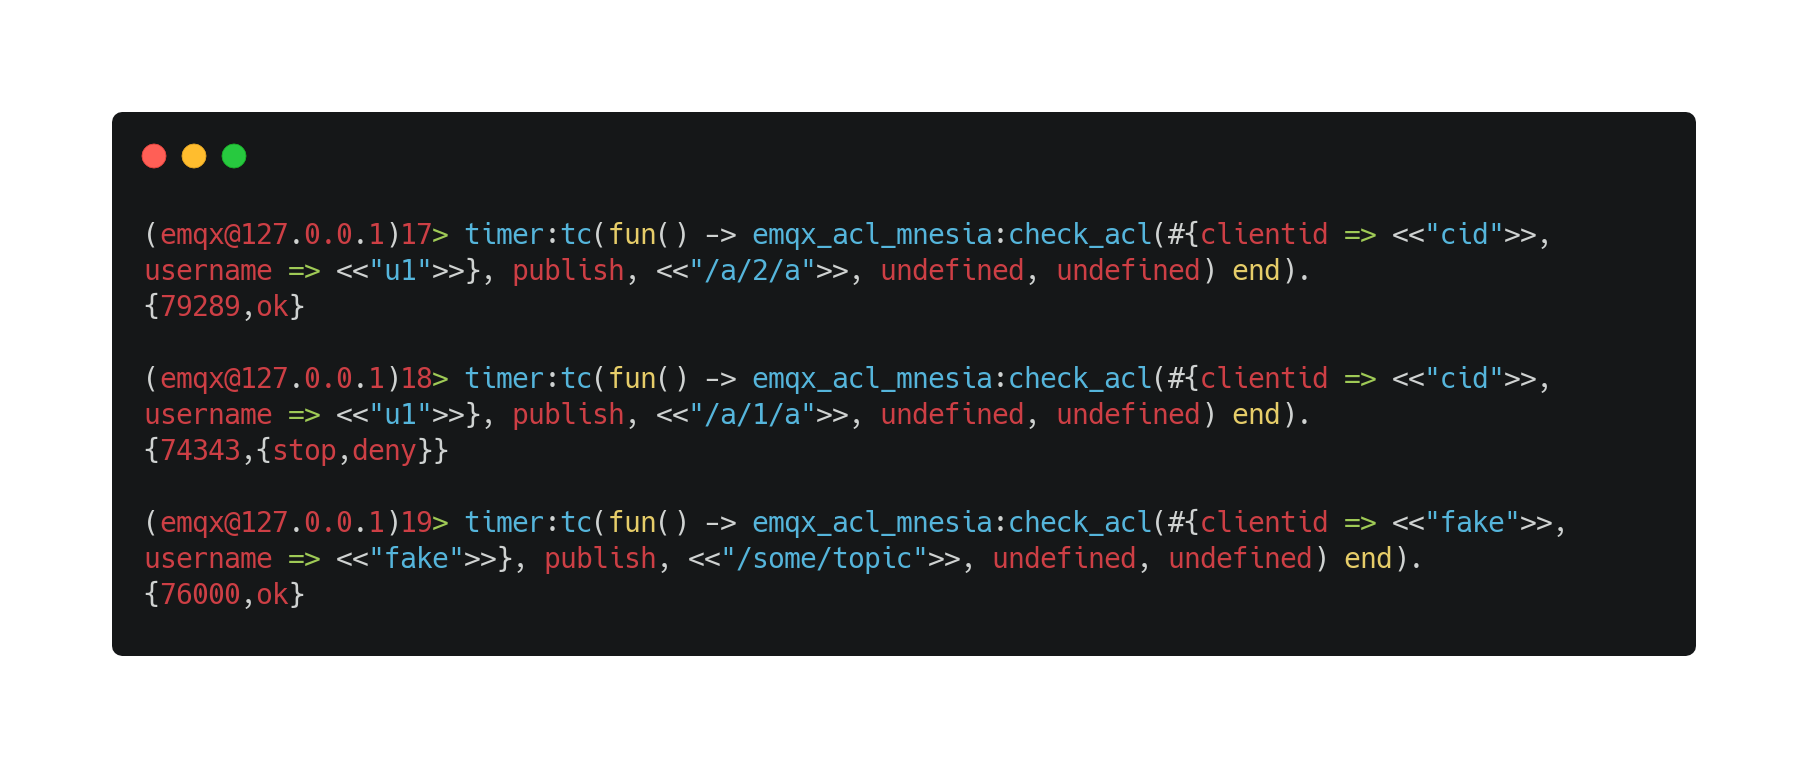
\includegraphics[width=10cm, keepaspectratio]{images/old-lookup-code-tc.png}
    \end{center}
\end{frame}

\begin{frame}
    \frametitle{How to fix?}

    \begin{itemize}
        \item Since table type is \textbf{bag} we can't use partial scans to take advantage of ordering
        \item Since there actually may be duplicates we can't somehow change \lstinline{ets} type for the table
    \end{itemize}
\end{frame}

\begin{frame}
    \frametitle{How to fix?}
    \framesubtitle{We need to change schema}

    \begin{itemize}
        \item We should have \lstinline{UserId} as key, like in 5.x or 4.2 branch
        \item The fix is easy
        \item But...
    \end{itemize}
\end{frame}

\begin{frame}
    \frametitle{How to fix?}
    \framesubtitle{We need to change schema on the fly}

    \begin{itemize}
        \item We should introduce optimization during cluster upgrade as well
        \item There may be present new nodes and old nodes in the cluster
        \item ACL rules can be added through \lstinline{emqx_ctl} or API on an \textbf{old} node, and \textbf{new}
        nodes should take them in account
        \item ACL rules can be added through \lstinline{emqx_ctl} or API on a \textbf{new} node, and \textbf{old}
        nodes should take them in account
    \end{itemize}
\end{frame}

\begin{frame}
    \frametitle{The plan}
    \framesubtitle{Migration part}

    We introduce a new \lstinline{migrator} process which is started during cluster upgrade or when a new node starts.
    \begin{itemize}
        \item It creates new \lstinline{emqx_acl2} table to eventually hold all ACLs from old \lstinline{emqx_acl} table
        \item Starts to check constantly wether \textbf{all nodes} of the cluster have \lstinline{migrator} processes
        \item When this is true, it \textbf{puts a tombstone} (a special record) into old \lstinline{emqx_acl} table
        \item Starts to move records from \lstinline{emqx_acl} to \lstinline{emqx_acl2}, each one in transaction. Several
        nodes may be doing this simultaneously
        \item Finally checks that the old \lstinline{emqx_acl} table is empty (has only the tombstone) and hibernates
    \end{itemize}
\end{frame}

\begin{frame}
    \frametitle{The plan}
    \framesubtitle{Perspective of ACL database client module}

    ACL database client module does not know about migration process, it knows only about the tombstone.
    While there is \textbf{no tombstone}, ACL database client
    \begin{itemize}
        \item Stores new ACL rules \textbf{both} into old \lstinline{emqx_acl} and new \lstinline{emqx_acl2} tables
        \item Removes ACL rules from \textbf{both} tables
        \item Retreives ACL rules from \textbf{both} tables and combines them
    \end{itemize}
    We need to have duplication because at this point
    there still may be nodes in the cluster knowing nothing about the new table.
\end{frame}

\begin{frame}
    \frametitle{The plan}
    \framesubtitle{Perspective of ACL database client module}

    When there is the \textbf{tombstone}, ACL database client
    \begin{itemize}
        \item Stores new ACL rules into the \textbf{new} \lstinline{emqx_acl2} only.
            Now there are no old nodes not knowing about \lstinline{emqx_acl2}.
        \item Removes ACL rules from both tables. This is no-op after the migration is over.
        \item Retrieves ACL rules from both tables and combines them. After the migration is over
            old table has no records, and this is also a no-op.
    \end{itemize}
\end{frame}

\begin{frame}
    \frametitle{The plan}
    \framesubtitle{\lstinline{appup}}

    \begin{center}
        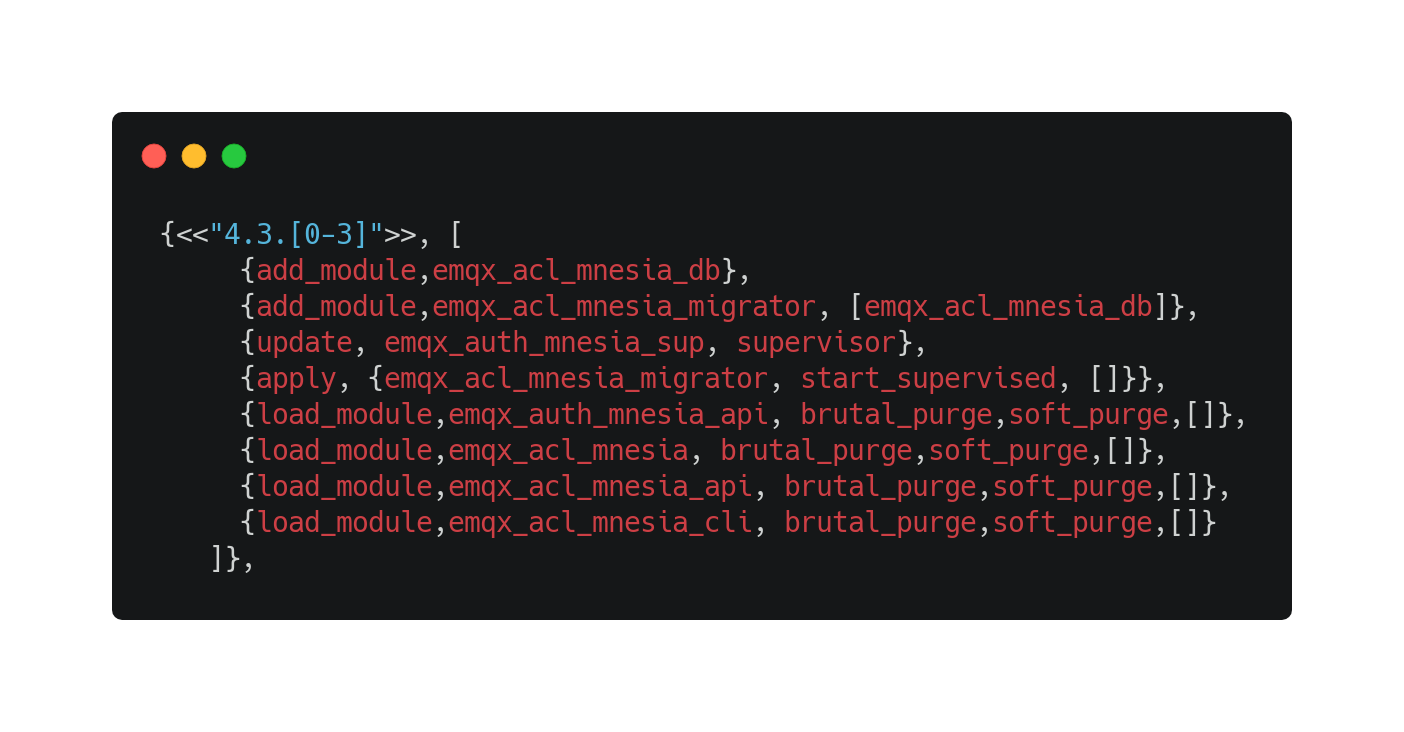
\includegraphics[width=10cm, keepaspectratio]{images/appup.png}
    \end{center}\end{frame}

\begin{frame}
    \frametitle{Local test}

    \begin{center}
        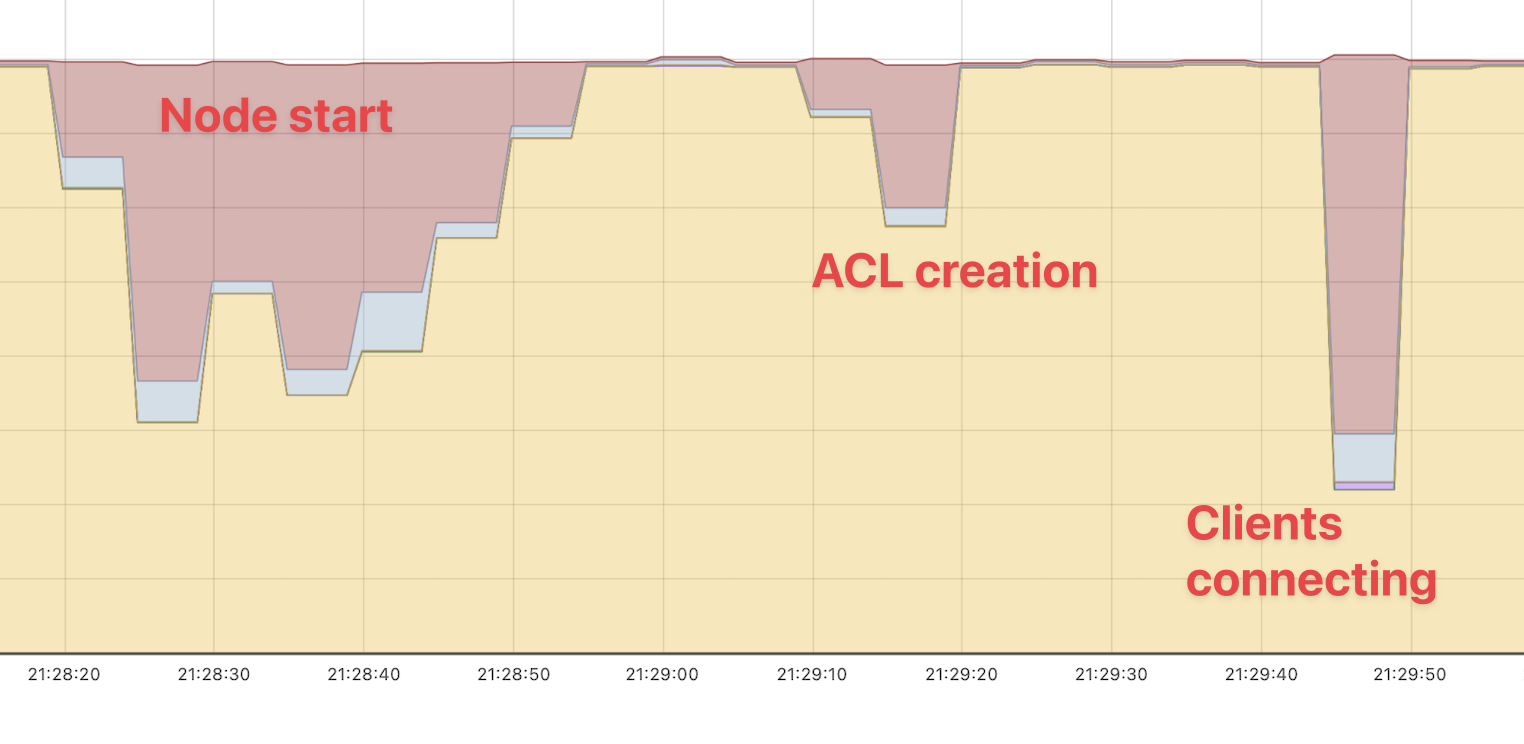
\includegraphics[width=10cm, keepaspectratio]{images/optimized.png}
    \end{center}
\end{frame}

\begin{frame}
    \frametitle{AWS Cluster test}

    \href{https://github.com/savonarola/emqx-acl-migration-test}{https://github.com/savonarola/emqx-acl-migration-test}
    \begin{itemize}
        \item Virtual environment created with \href{https://github.com/qzhuyan/cdk-emqx-cluster}{EMQX CDK}
        \item 5 nodes
        \item 100000 connected clients
        \item 100000 ACL records
    \end{itemize}
\end{frame}

\begin{frame}
    \frametitle{AWS Cluster test}

    \begin{center}
        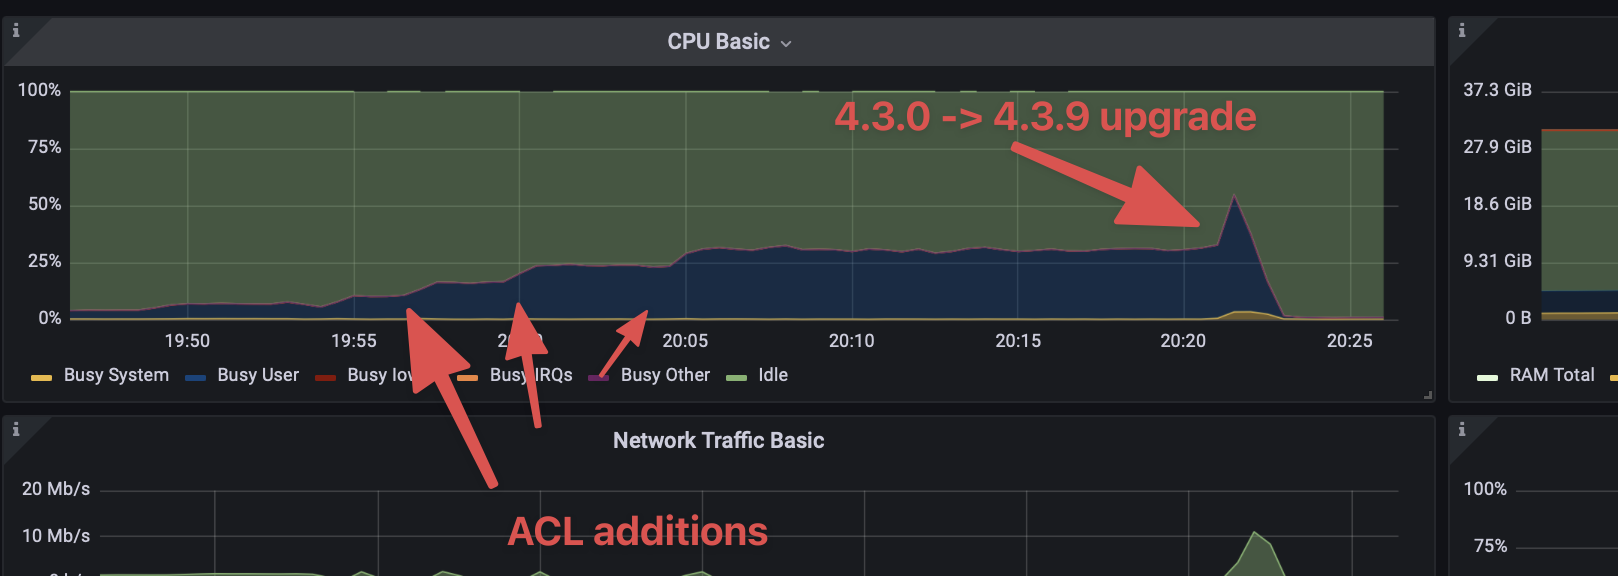
\includegraphics[width=10cm, keepaspectratio]{images/optimized-cluster.png}
    \end{center}
\end{frame}

\begin{frame}
    \frametitle{AWS Cluster test}

    \begin{itemize}
        \item The more ACL records we have, the more CPU is consumed by pubs,
            even though ACL records are not related to the publishing clients
        \item We have a CPU consumption peak during migration
        \item CPU usage is greatly reduced after the migration
    \end{itemize}
\end{frame}

\begin{frame}
    \frametitle{AWS Cluster test}

    \begin{center}
        Thank you!
    \end{center}
\end{frame}

\end{document}
